\documentclass{beamer}
\usepackage{caption}
\usepackage{subfigure}
\usetheme[background=light]{metropolis}

\title{A Presentation of our Work}
\date{2016-08-18}
\author{The Swedish Interns}
\institute{Created for NVI Inc. at the Goddard Space Flight Centre}

\begin{document}
    \maketitle

    \begin{frame}{Table of Contents}
    \tableofcontents
    \end{frame}

%%%%%%%%%%%%%%%%%%%%%%%%%%%%%%%%%%%%%%%%%%%%%%%%%%%%%%%%%%%%%%%%%%%%%%%%%%%%%%%

    \section{Weeks 1-2: Learning Fortran}

    \begin{frame}{Calculator}
        \begin{figure}[ht]
            \centering
            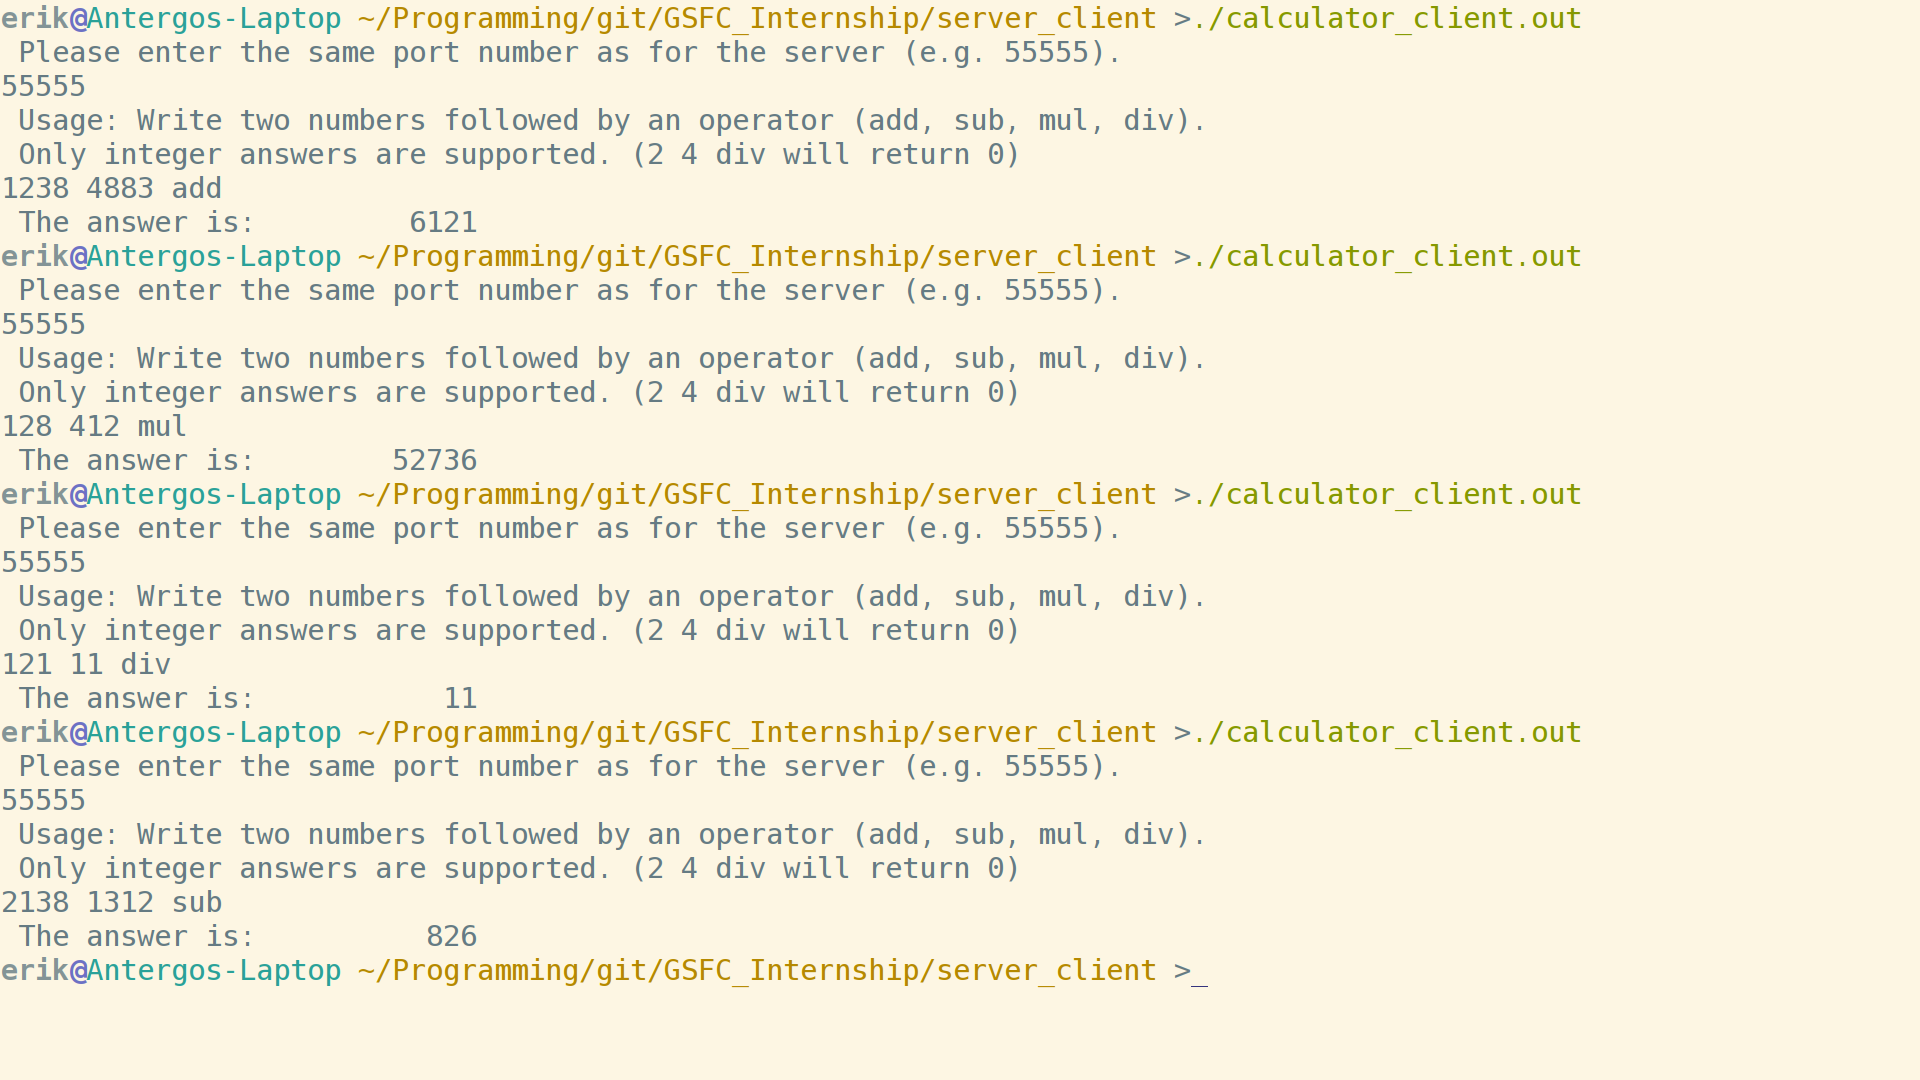
\includegraphics[width=1\columnwidth]{calculator}
            \caption{Example usage of the TCP calculator.}
        \end{figure}
    \end{frame}

%%%%%%%%%%%%%%%%%%%%%%%%%%%%%%%%%%%%%%%%%%%%%%%%%%%%%%%%%%%%%%%%%%%%%%%%%%%%%%%

    \section{Weeks 3-7: Our First Project}

    \begin{frame}{Problem Description}
        Rewrite how globl/solve handles its passing of data to and from
        usrpartials and usrprogs.

        By minimizing disc I/O we want to increase the speed at which data is
        sent.
    \end{frame}

%%%%%%%%%%%%%%%%%%%%%%%%%%%%%%%%%%%%%%%%%%%%%%%%%%%%%%%%%%%%%%%%%%%%%%%%%%%%%%%
    \section{Week 3-4: Testing I/O performance}

    \begin{frame}{I/O Performance}
    \begin{itemize}[<+-|alert@+>]
        \item A couple of contenders:
            \begin{itemize}
                \item Read/Write with files
                \item Read/Write with pipes
                \item Sending/Receiving with TCP Sockets
                \item Sending/Receiving with OpenMPI
                \item Sending/Receiving with ZeroMQ
            \end{itemize}
    \end{itemize}
    \end{frame}
%%
    \begin{frame}{Performance Test}
        \begin{enumerate}[<+-|alert@+>]
            \item The producer generates a list of length n and fills it with
                  integers.
            \item The producer writes the list to file (or sends it over the
                  designated transfer protocol).
            \item The consumer reads (or receives) the list.
            \item The consumer squares each int in the list and sends it back
                  to the producer.
            \item The producer reads (or receives) the modified list.
        \end{enumerate}
    \end{frame}
%%
    \begin{frame}{Result for I/O Performance}
    \begin{figure}[h!]
        \centering
        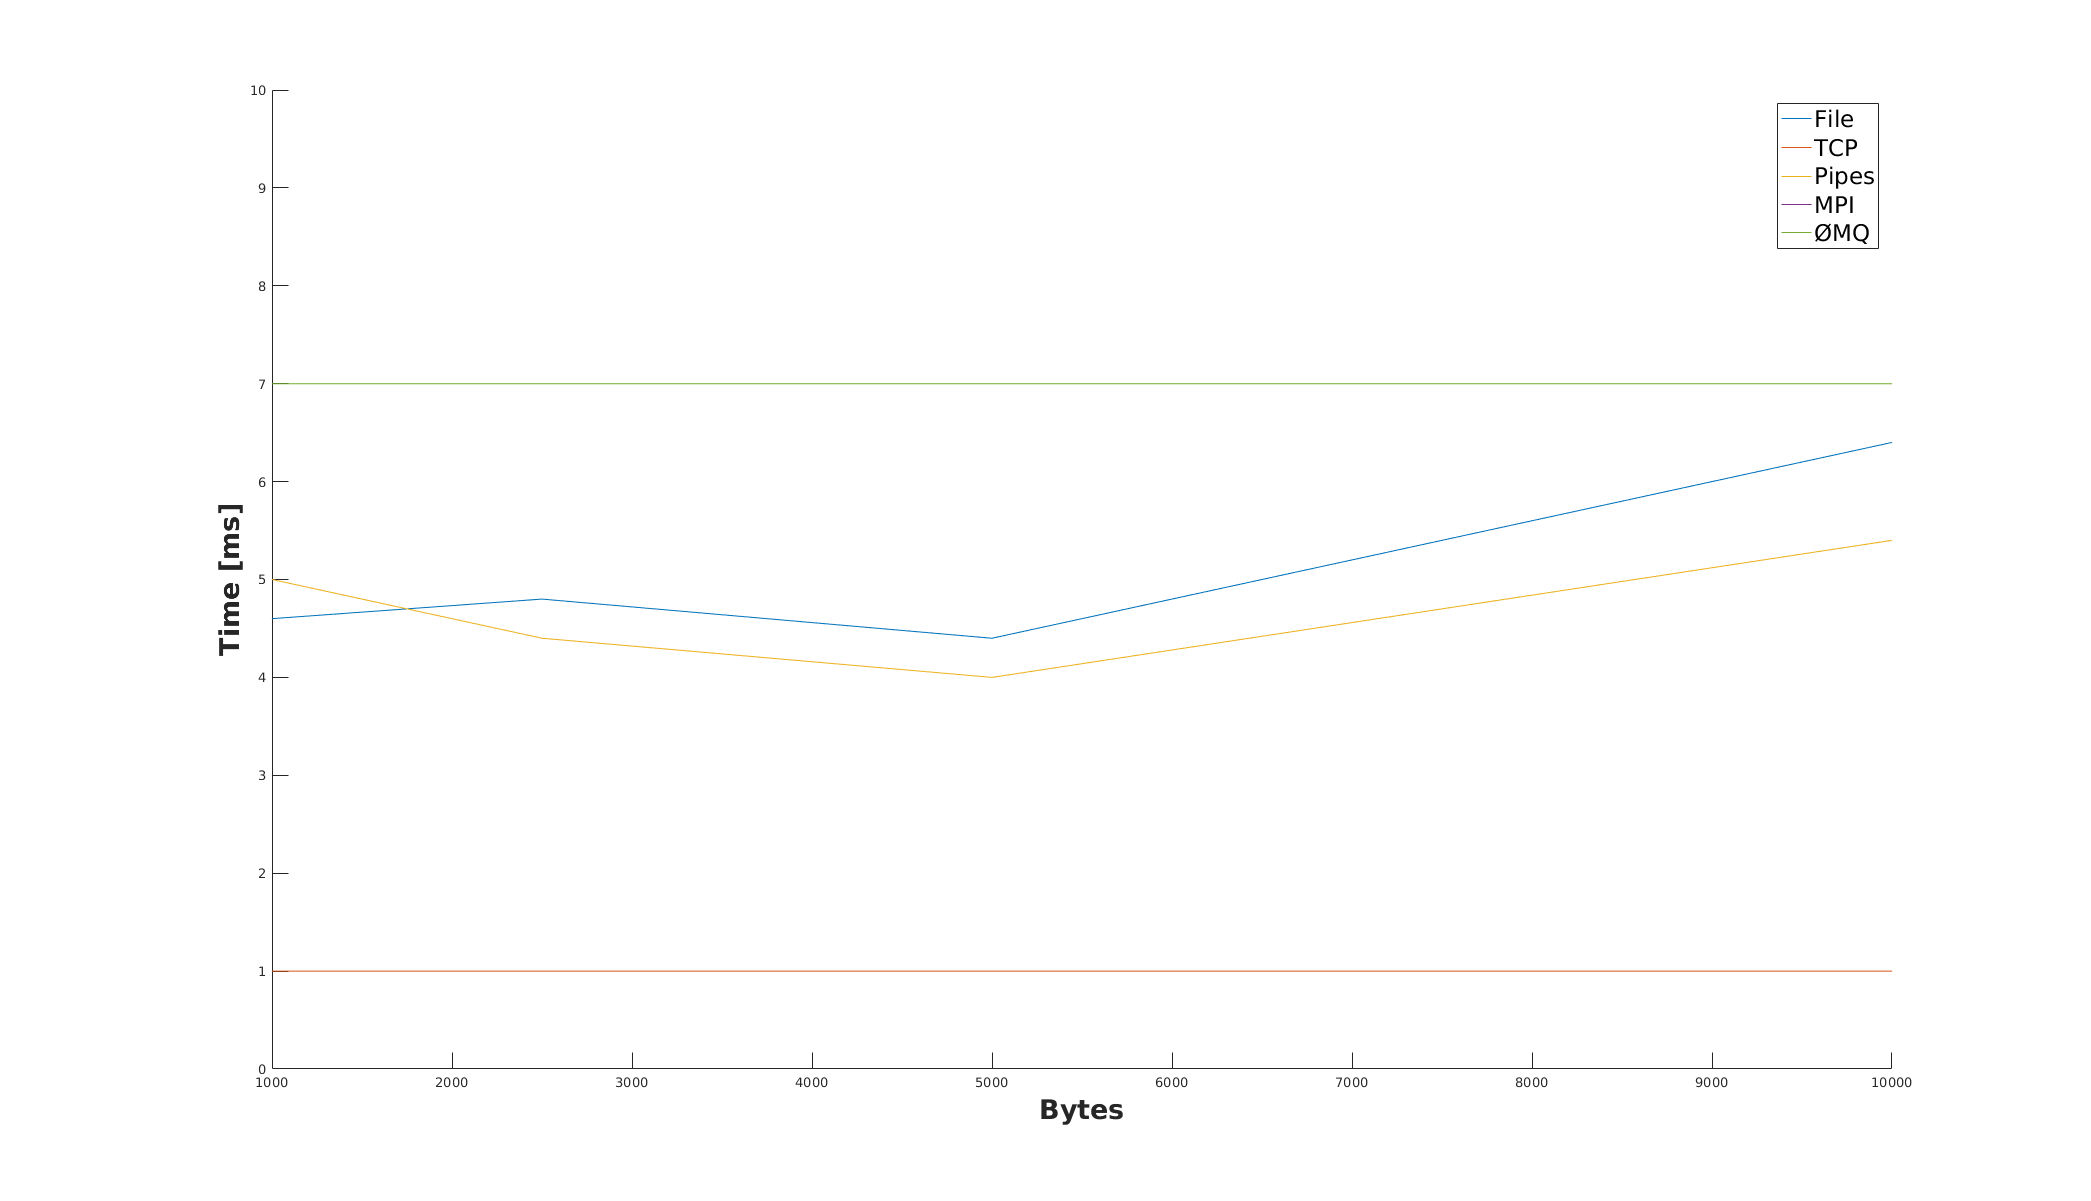
\includegraphics[width=1\columnwidth]{singlerun-nf}
    \end{figure}
    \end{frame}
%%
    \begin{frame}
    \begin{figure}[h!]
        \centering
        \includegraphics[width=1\columnwidth]{thousandrun+file}
    \end{figure}
    \end{frame}
%%
    \begin{frame}{Result for I/O Performance}
    \begin{figure}[h!]
        \centering
        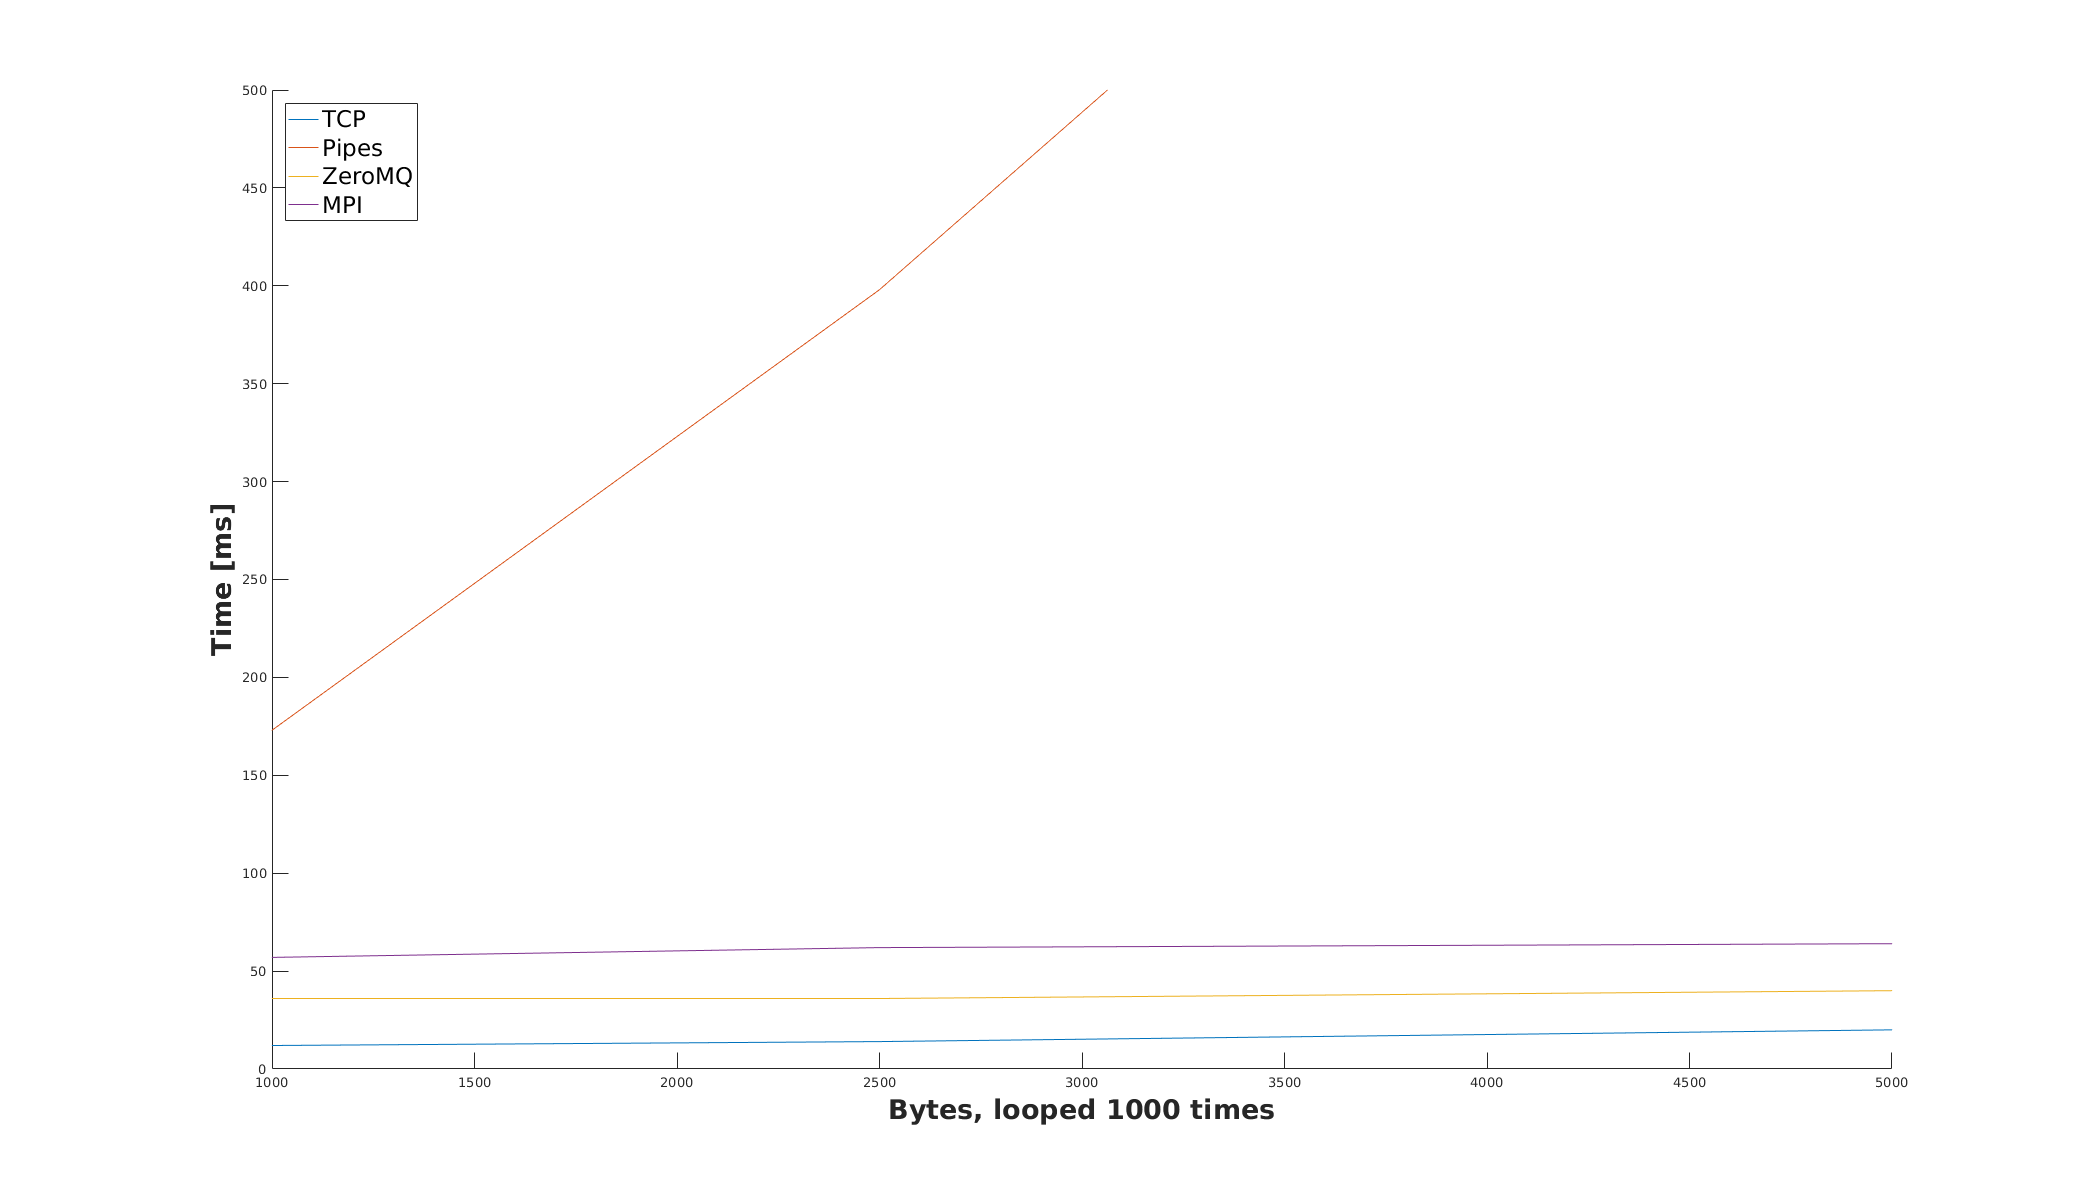
\includegraphics[width=1\columnwidth]{thousandrun-nf}
    \end{figure}
    \end{frame}
%%
    \begin{frame}{Result for I/O Performance}
    \begin{itemize}[<+-|alert@+>]
        \item TCP was the fastest, but the most difficult to implement.
        \item Since we assumed a lot of data would be passed we opted for ZeroMQ
              due to its presumptive ease of use and performance.
    \end{itemize}
    \end{frame}

%%%%%%%%%%%%%%%%%%%%%%%%%%%%%%%%%%%%%%%%%%%%%%%%%%%%%%%%%%%%%%%%%%%%%%%%%%%%%%%

    \section{Weeks 5-7: Implementation}

    \begin{frame}{Implementation}
    \begin{itemize}[<+-|alert@+>]
        \item Installation of Software on \bf{bootes}
        \item Porting our code to ifort
        \item A lot of coding
    \end{itemize}
    \end{frame}

%%%%%%%%%%%%%%%%%%%%%%%%%%%%%%%%%%%%%%%%%%%%%%%%%%%%%%%%%%%%%%%%%%%%%%%%%%%%%%%

    \section{Results for Project One}

    \begin{frame}{Results for Project One}
        Running userpartials for ~200 observations.\\
        Old version of globl/solve: 8 minutes 47 seconds\\
        New version of globl/solve: 9 minutes 5 seconds
    \end{frame}
%%
    \begin{frame}{Results for Project One}
        \centering{Why?}
    \end{frame}
%%
    \begin{frame}{Results for Project One}
        Globl/solve does not read and write a lot, it reads a lot,
        \centering
        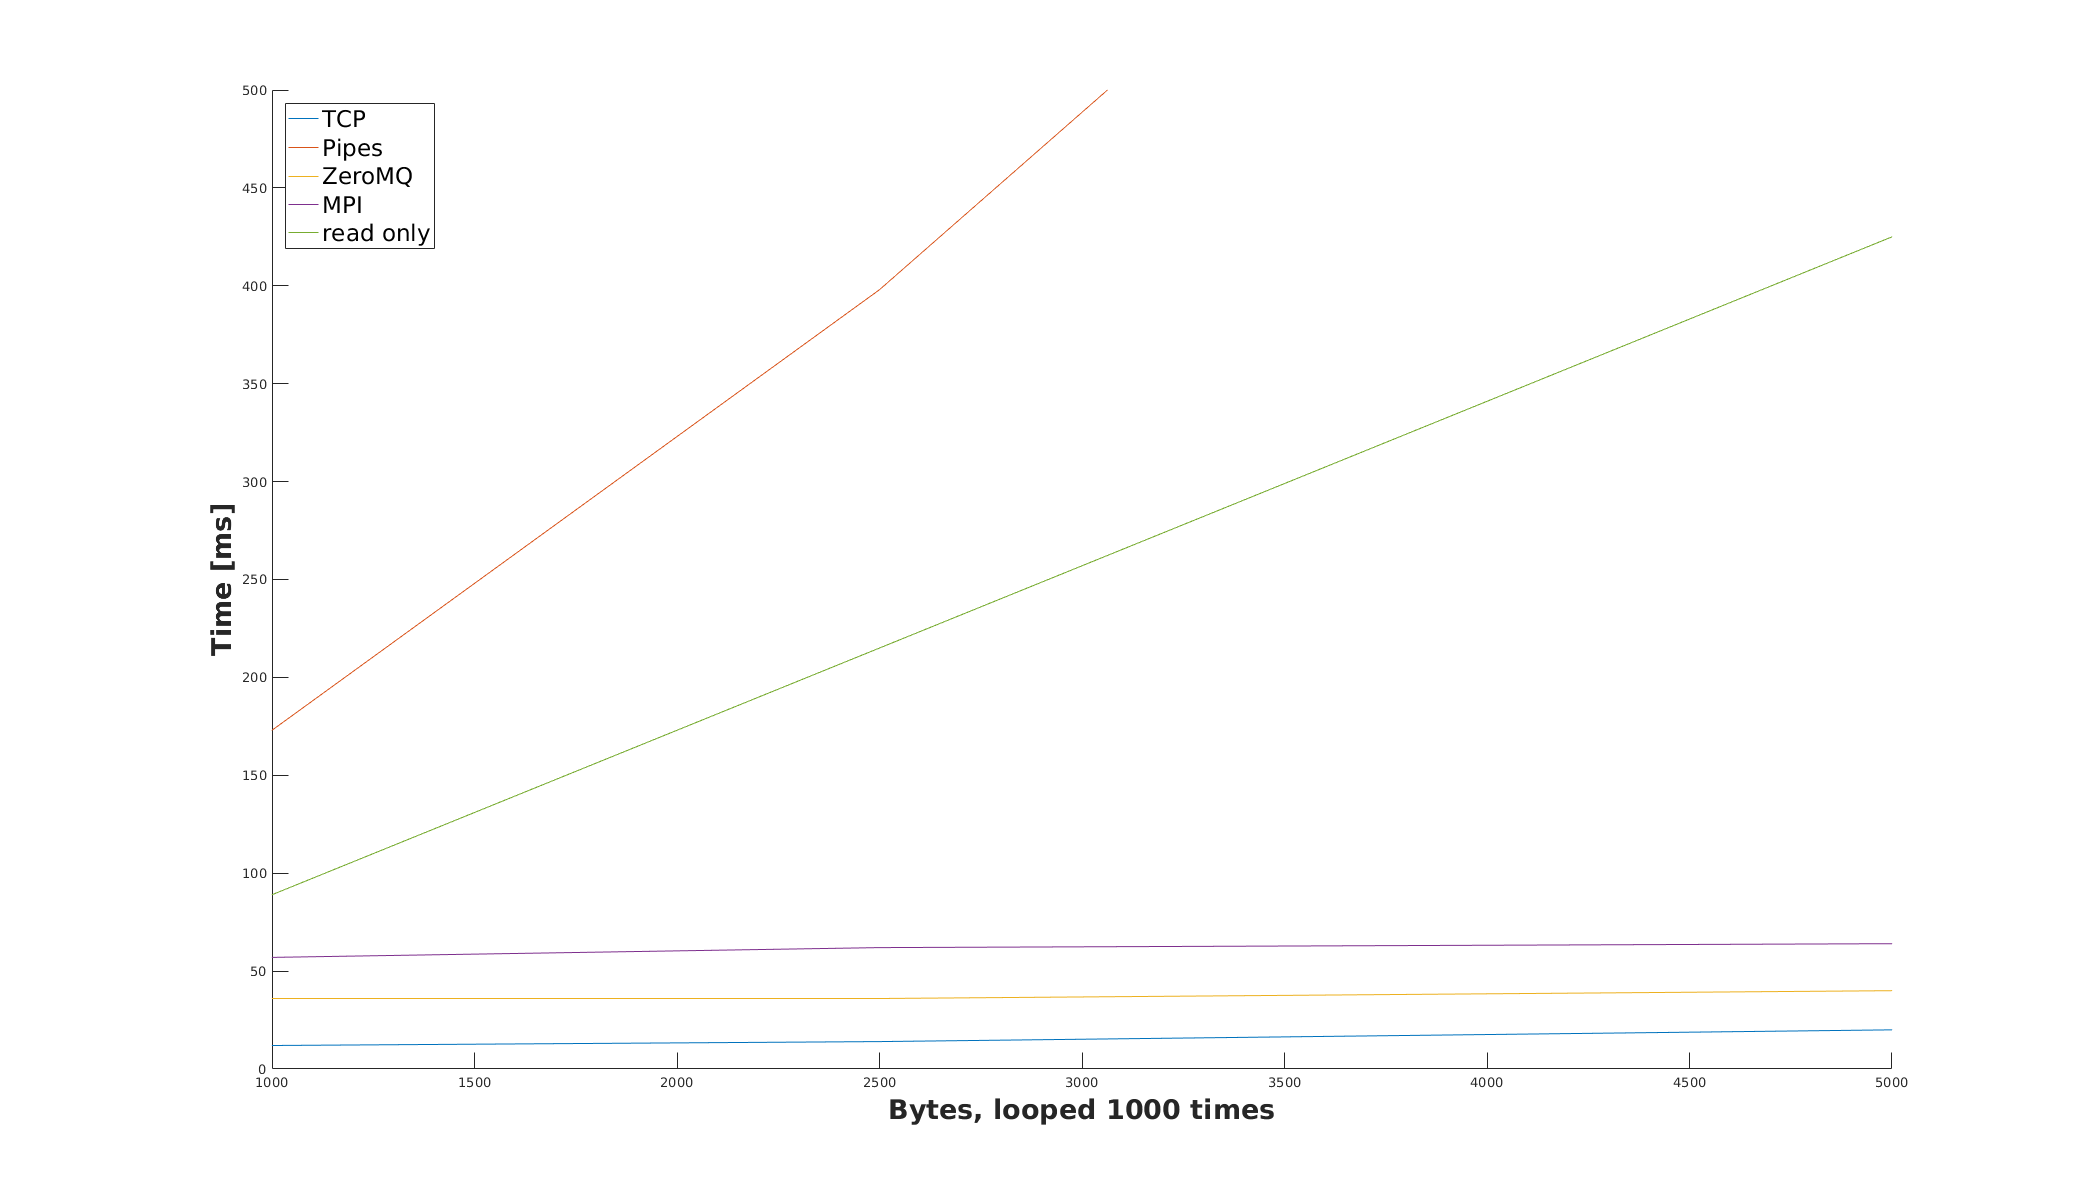
\includegraphics[width=1\columnwidth]{thousandrun}

        but read only is still slower...
    \end{frame}
%%
    \begin{frame}{Results for Project One}
        Globl/solve does not read as much as we thought,
        \centering
        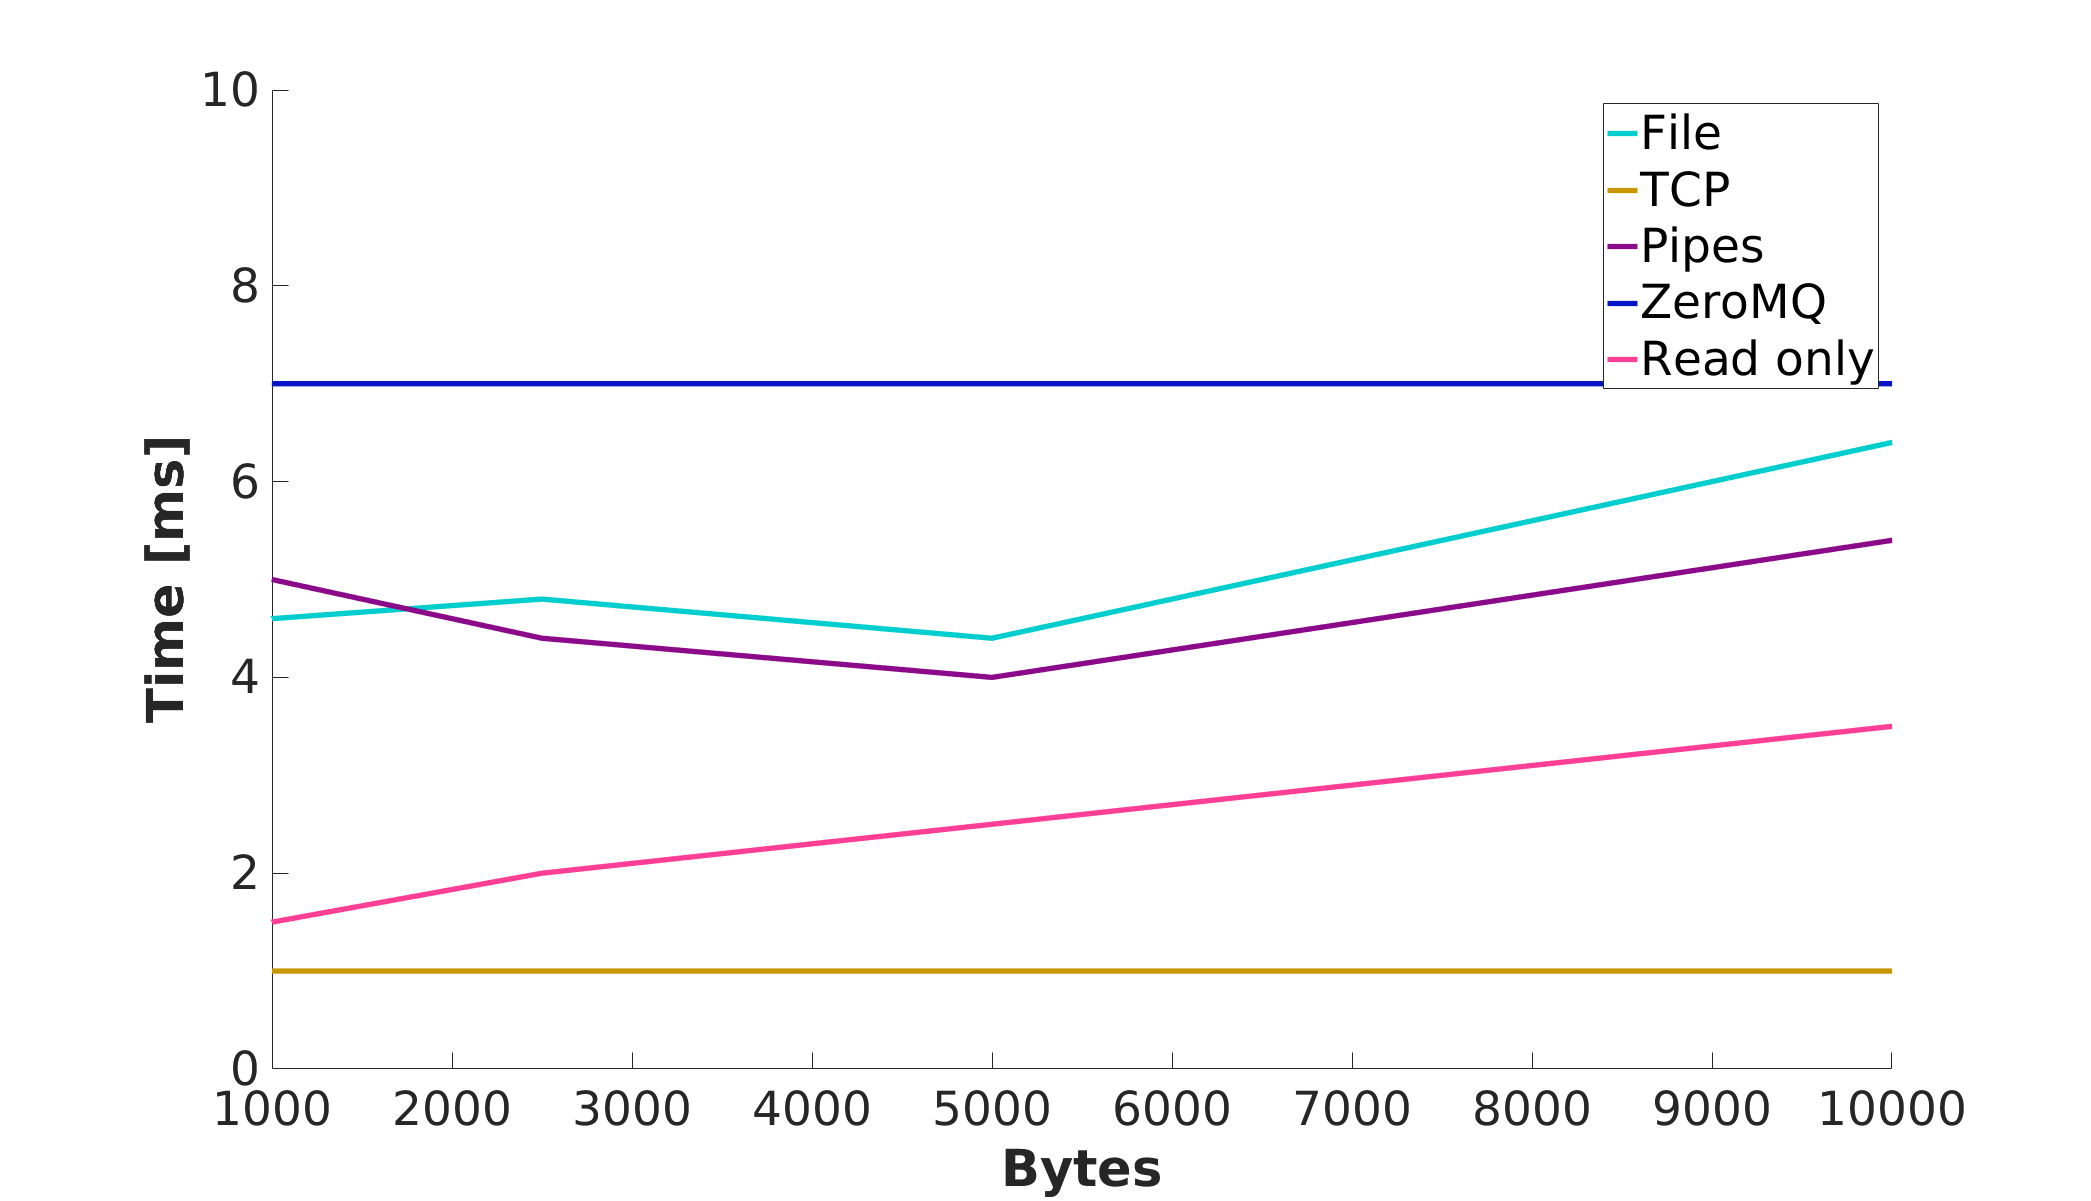
\includegraphics[width=1\columnwidth]{singlerun}
    \end{frame}
%%
    \begin{frame}{Future studies}
        \begin{itemize}[<+-|alert@+>]
            \item Remove the writes that are no longer needed.
            \item TCP should have been the way to go?
            \item Posix Shared Memory? Conversion between C and Fortran was non trivial.
        \end{itemize}
        \centering
        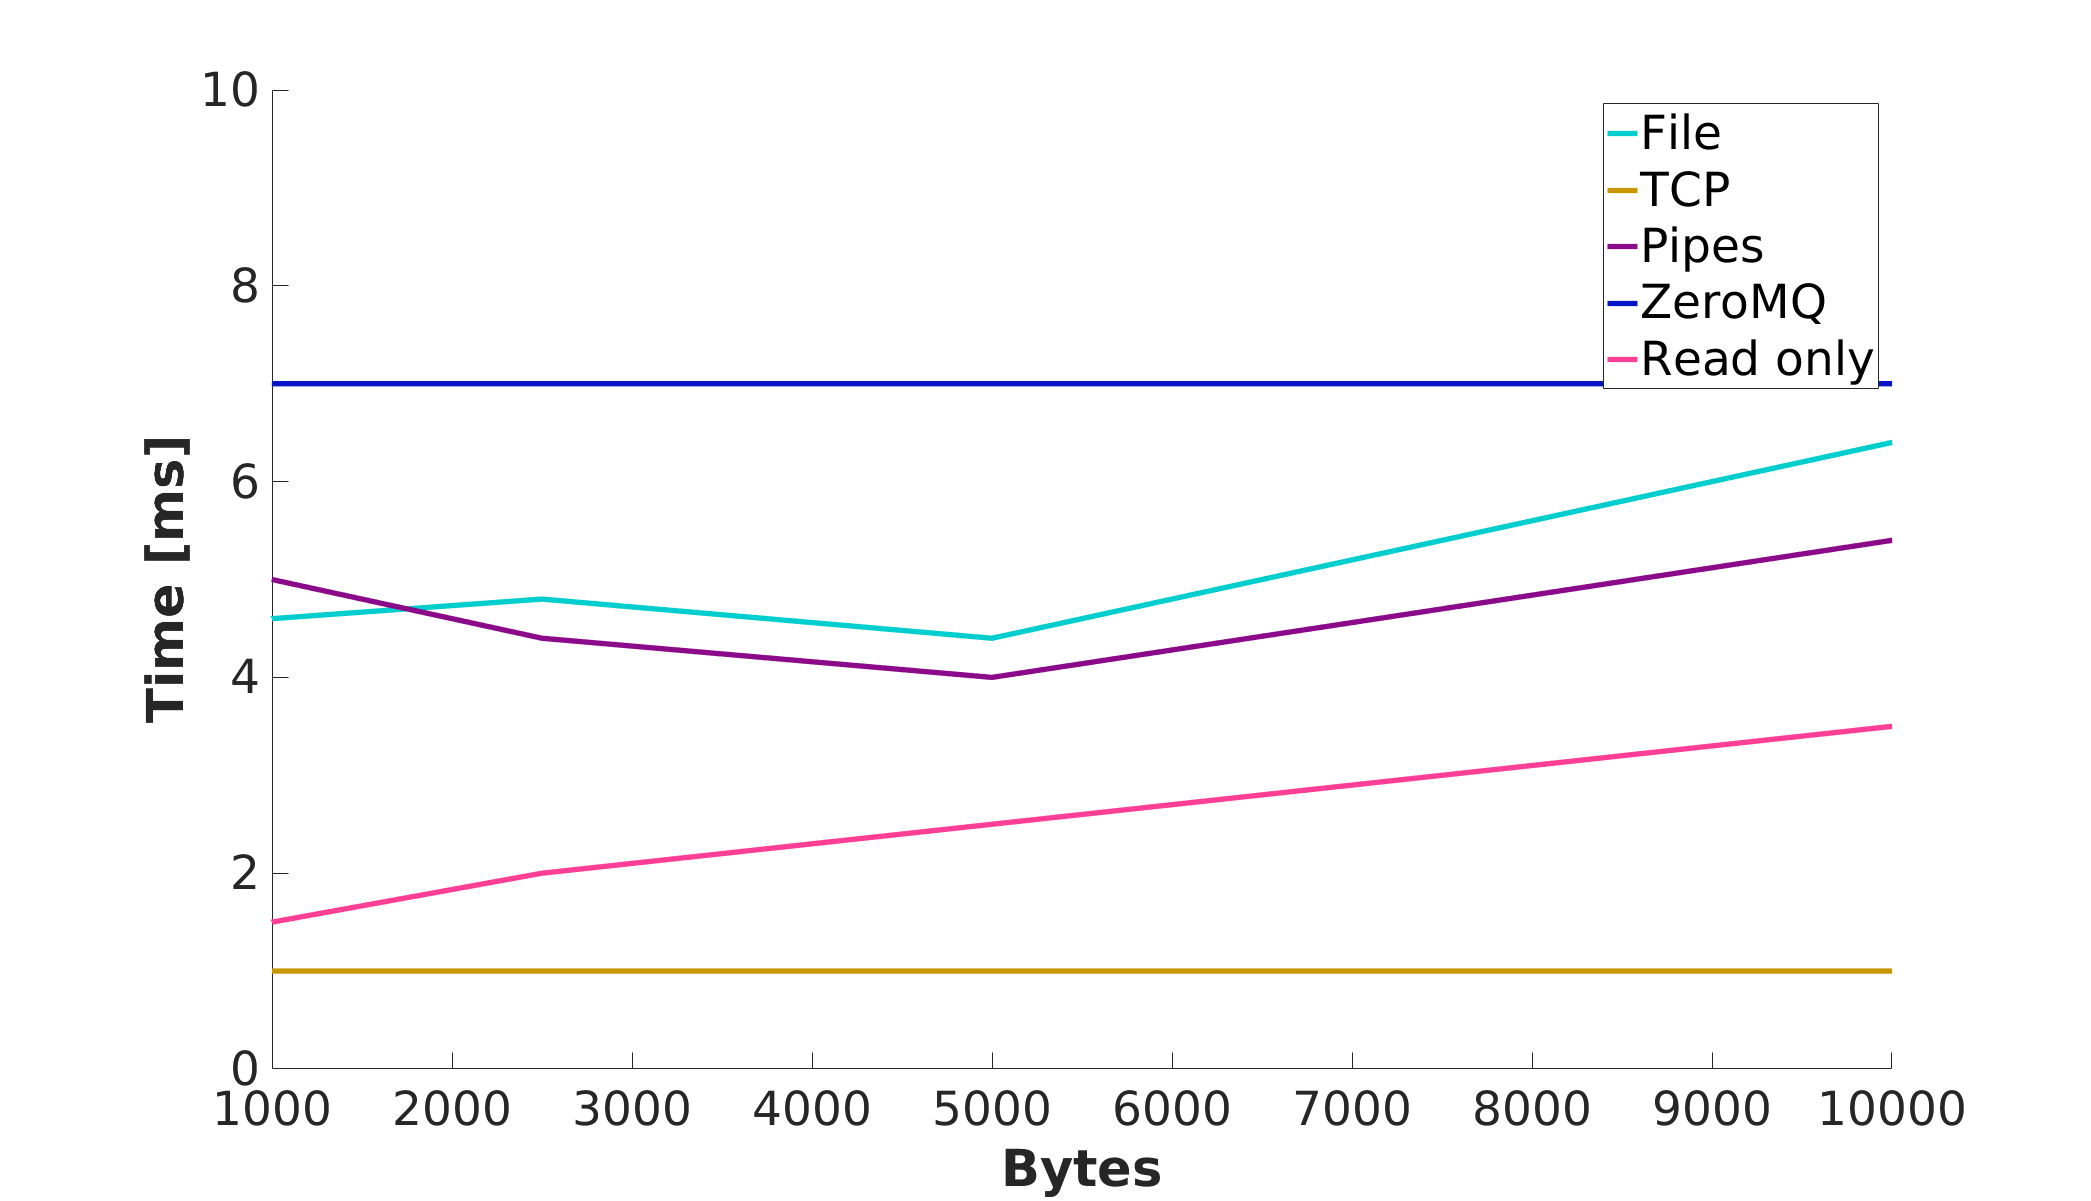
\includegraphics[width=1\columnwidth]{singlerun}
    \end{frame}

%%%%%%%%%%%%%%%%%%%%%%%%%%%%%%%%%%%%%%%%%%%%%%%%%%%%%%%%%%%%%%%%%%%%%%%%%%%%%%%

    \section{Weeks 7-9: Our Second Project}

    \begin{frame}{Problem Description}
        The model used for determining when an antenna acquires a source is a
        little bit off. Sked will say that an antenna should be on target at
        time $T$ but the logfiles tells us that the antenna actually was on
        source at $T \pm c$.
    \end{frame}
%%
    \begin{frame}{Extract the Data}
        \centering
        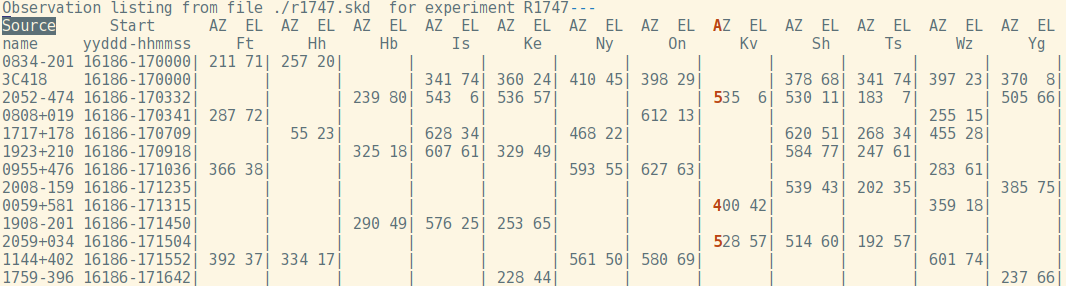
\includegraphics[width=1\columnwidth]{skds}\\[2ex]
        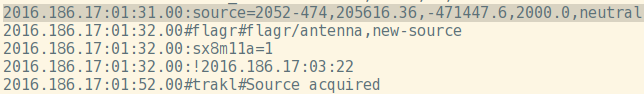
\includegraphics[width=0.75\columnwidth]{logs}
    \end{frame}
%%
    \begin{frame}{Parse the Data}
        \begin{itemize}[<+-|alert@+>]
            \item Correlate the log data with the Sked data.
            \item Least Square Fit
            \begin{itemize}[<+-|alert@+>]
                \item Iteratively re calculate to get rid of noise.
            \end{itemize}
        \end{itemize}
    \end{frame}

%%%%%%%%%%%%%%%%%%%%%%%%%%%%%%%%%%%%%%%%%%%%%%%%%%%%%%%%%%%%%%%%%%%%%%%%%%%%%%%

    \section{Result for Project Two}

    \begin{frame}{Result for Project Two}
        \centering
        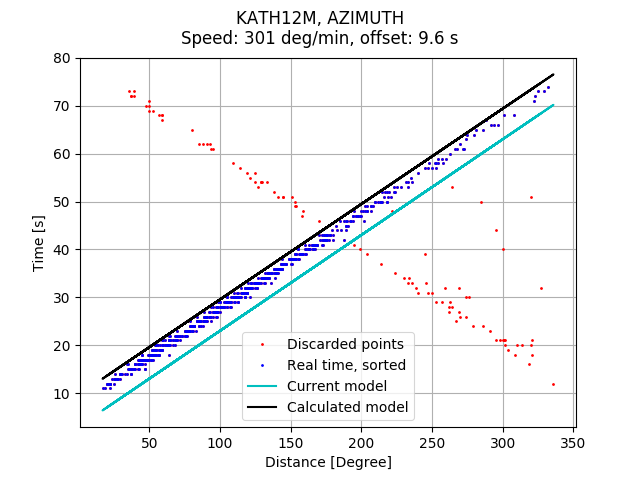
\includegraphics[width=1\columnwidth]{ke_az}
    \end{frame}
%%
    \begin{frame}{Future studies}
        \begin{itemize}[<+-|alert@+>]
            \item Fix the bug in Sked.
            \item Set a more intelligent threshold.
        \end{itemize}
    \end{frame}

%%%%%%%%%%%%%%%%%%%%%%%%%%%%%%%%%%%%%%%%%%%%%%%%%%%%%%%%%%%%%%%%%%%%%%%%%%%%%%%

    \section{Week 10: Returning Home}

    \begin{frame}{Returning Home}
        During our time here we have:
        \pause
        \begin{itemize}[<+-|alert@+>]
            \item been exposed to how it is to work at NASA and NVI.
            \item learned the importance of conducting thorough research.
            \item realized that patience really is a virtue...
        \end{itemize}
    \end{frame}

    \begin{frame}{Returning Home}
        \centering
        Thank you! \\ [2ex]
        \includegraphics[width=1\columnwidth]{interns}
    \end{frame}

\end{document}

